\documentclass{article}[a4paper]
\usepackage[utf8]{inputenc}
\usepackage[spanish]{babel}
\usepackage[a4paper, 11pt]{geometry}
\usepackage{graphicx}
\newcommand{\xor}{\oplus}
\usepackage{xcolor}
\usepackage{listings} %code highlighter
\usepackage{blindtext}
\usepackage{titlesec}
\usepackage{appendix}
\usepackage[T1]{fontenc}
\usepackage{textcomp}
\usepackage{amssymb,amsmath}
\usepackage{hyperref}

\newcommand\tab[1][1cm]{\hspace*{#1}}

\definecolor{codegreen}{rgb}{0,0.6,0}
\definecolor{codegray}{rgb}{0.5,0.5,0.5}
\definecolor{codepurple}{rgb}{0.58,0,0.82}
\definecolor{backcolour}{rgb}{0.95,0.95,0.92}

\lstdefinestyle{mystyle}{
    backgroundcolor=\color{backcolour},   
    commentstyle=\color{codegreen},
    keywordstyle=\color{magenta},
    numberstyle=\tiny\color{codegray},
    stringstyle=\color{codepurple},
    basicstyle=\ttfamily\footnotesize,
    breakatwhitespace=false,         
    breaklines=true,                 
    captionpos=b,                    
    keepspaces=true,                 
    numbers=left,                    
    numbersep=5pt,                  
    showspaces=false,                
    showstringspaces=false,
    showtabs=false,                  
    tabsize=2
}

\lstset{style=mystyle}

\title{Memoria Práctica PDL}
\author{Andrés Ollero Morales, Gabriel de Oliveira Trindade, Víctor Alejandro Sanz Ararat}
\date{Grupo 17}

\begin{document}

\maketitle
\thispagestyle{empty}
\newpage
\tableofcontents
\thispagestyle{empty}

\newpage

\section{Diseño del Analizador Léxico}

\subsection{Diseño de Tokens}
\begin{verbatim}
        <palabraReservada, boolean>         <palabraReservada, input>
        <palabraReservada, break>           <palabraReservada, int>
        <palabraReservada, case>            <palabraReservada, let>
        <palabraReservada, function>        <palabraReservada, switch>
        <palabraReservada, print>           <palabraReservada, return>
        <palabraReservada, string>          <palabraReservada, if>
        
        <suma, >            <puntoComa, >       <asignacion, >
        <negacion, >        <coma, >            <dosPuntos, >
        <abrePar, >         <cierraPar, >       <comparacion, >
        <abreLlave, >       <cierraLlave, >     <asignacionResto, >
        <id, nºTS>          <constEnt, nº>      <cadena, "lexema">
\end{verbatim}

\subsection{Gramática}
\begin{verbatim}
    S -> "A | dB | %C | =D | _T | cT | {  |  }  |  (  |  )  |  +  |
          :  |  ;  |  ,  |  ! | del S
    T -> cT | _T | dT | O.C 
    A -> lA | " 
    B -> dB | O.C
    C -> =
    D -> = | O.C
    E -> \ E' | O.C
    E’ -> *E" | O.C E
    E’’ -> \ | O.C E'
    
    donde c = letras (a-z, A-Z), d = dígitos (0-9), l = cualquier cosa 
    y O.C = otro caracter distinto
\end{verbatim} 

%AÑADIR SIMBOLO XOR!!!!!!!!!!!!!!!!!!!!!!!!!!!!!!!!!!!!!!!!!!!!!!!!!!!!!!!!!!!!!!!!!!!!!!!!!!!!
\subsection{Acciones Semánticas}
Se realiza la acción semántica LeerSigCaracter en todas las transiciones 
menos en las transiciones:
\begin{verbatim}
T : 101
B : 103
D : 105
S : T -> lexema = l ; contador = 1;
T : T -> lexema = lexema CONCATENAR l ; contador++
T : 101 -> if (BuscarPalabraReservada(lexema) == 1) 
                then GenerarToken(palabraReservada, “”)
            else if (BuscarTablaSimbolos(lexema) == 1) 
                then GenerarToken(id, posTS)
            else (BuscarTablaSimbolos(lexema) == 0) 
                then AñadirEntradaTabla(id, posTS) &&
                        GenerarToken(palabraReservada, posTS);
S : A -> contador = 0; lexema = ""
A : A -> lexema = lexema CONCATENAR l ; contador++;
A : 102 -> if (contador <= 64) 
                then GT(cadena, lexema)
	            else 
	                then printf(“Error, longitud de la cadena excede el limite”)
S : B -> valor = valor_ascci(d);;
B : B -> valor = valor + valor_ascci(d);
B : 103 -> if (valor <= 32767) 
                then GT (constEnt, valor)
	            else
	                then Printf(“Error, valor del entero excede el limite”)
C : 104 -> if (c != ‘=’)
                then Printf(“Error : Expected '%=”)
           else 
                GenerarToken(asignacionResto, )
D : 105 -> GenerarToken(igual, );
D : 106 -> GenerarToken(comparación, );
S : 107 -> GenerarToken(abreLlave, );
S : 108 -> GenerarToken(cierraLlave, );
S : 109 -> GenerarToken(abrePar, );
S : 110 -> GenerarToken(cierraPar, );
S : 111 -> GenerarToken(dosPuntos, );
S : 112 -> GenerarToken(puntoComa, );
S : 113 -> GenerarToken(coma, );
S : 114 -> GenerarToken(negación, );
S : 115 -> GenerarToken(suma, );

- GenerarToken (atributo, valor): Genera el token en un fichero de 
                                  salida tokens.txt.
- BuscarPalabraReservada (lexema): Busca la palabra reservada en la 
                                   respectiva tabla de palabras reservada.
- AñadirEntradaTabla(lexema, posTS): Añadimos el nombre de la variable a 
                                     la tabla de símbolos.

\end{verbatim}

\subsection{Errores}
Cuando se introduce en el código un símbolo que no pertenece al lenguaje, nuestro autómata lo omite. Los errores que contempla el código son cuando (y su correspondiente mensaje por línea de comandos):\\

- Se crea un identificador que no empieza por letra o subrayado.
\tab \tab \textcolor{red}{Error : inicio de nombre de variable invalido.}

- Se introduce un número entero superior a 32767\\
\tab \tab \textcolor{red}{Error en línea: n -> Error Léxico: el valor numerico introducido excede el limite de 32767.}

- Se intenta crear una cadena de más de 64 caracteres\\
\tab \tab \textcolor{red}{Error en línea: n -> Error Léxico: Cadena sobrepasa los 64 caracteres.}

- Se crea una cadena sin finalizar con la doble comilla final\\
\tab \tab \textcolor{red}{Error: La string esta mal formada}\\

- Se introduce exclusivamente un '\%' sin el caracter '=' a continuación\\
\tab \tab \textcolor{red}{Error: Expected '=' after '\%'.}

- Se intenta hacer comentario de bloque y no se introducen los /* */ correctamente.\\
\tab \tab \textcolor{red}{Error en línea: n -> Error Léxico: Comentario mal formado, el fin debe tener la forma *\\.}\\

Y por supuesto, no se genera el token.

\subsection{Autómata Finito Determinista}
\begin{figure}[h!]
\centering
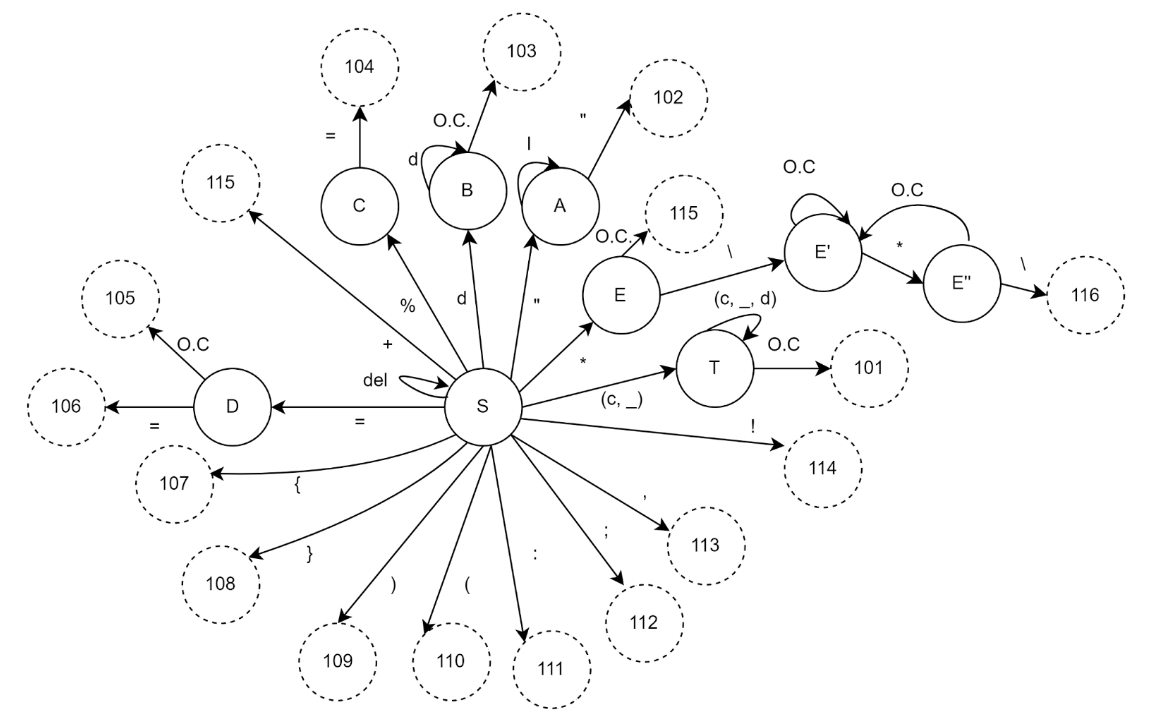
\includegraphics[width=0.9\textwidth]{automataAnLex.png}
\caption{\label{figura:automata}Implementación de la gramática con el autómata.}
\end{figure}

\section{Diseño inicial de la Tabla de Símbolos}

Cuando añadimos un identificador a la Tabla de Símbolos, primero comprobamos que no haya sido introducido previamente, y sino lo metemos. En el atributo del identificador pondremos el número que ha sido asignado, que en nuestro caso es el tamaño de la tabla en ese momento.\\

Decidimos que la mejor forma de implementar la Tabla de Símbolos era con la clase HashMap, que nos proporciona una búsqueda con complejidad constante, que a la hora de código con muchos identificadores la eficacia aumenta. El método de inserción para la clase es aleatorio por construcción, por tanto no tiene orden interno.

\section{Diseño del Analizador Sintáctico}
\subsection{Gramática}
Para ello hemos tomado la gramática que venía dada en las diapositivas de la explicación de la práctica modificándola a los terminales que escogimos al inicio. Eliminamos la recursividad por la izquierda y la factorizamos para cumplir la condición LL(1).

\begin{verbatim}
Axioma = P

NoTerminales = { P S SS E R RR U UU V VV L Q X B T A K C F H O D }

Terminales = { ! == + id ( ) constEnt cadena %= print input return , if break 
switch case int boolean string let function ; : = { } default }

Producciones = {
    	E -> ! R
    	E -> R 
    	R -> U RR
    	RR -> + R
    	RR -> lambda
    	U -> V UU
    	UU -> lambda
    	UU -> == U
    	V -> id VV
    	V -> ( E )
    	V -> constEnt
    	V -> cadena
    	VV -> ( L )
    	VV -> lambda
    	S -> id SS
    	SS -> %= E ; 
    	SS -> = E ;
    	SS -> ( L ) ;
    	S -> print R ;
    	S -> input id ;
    	S -> return X ;
    	L -> E Q
    	L -> lambda
    	Q -> , E Q
    	Q -> lambda
    	X -> E
    	X -> lambda
    	B -> switch ( E ) { O }
    	B -> if ( E ) S 
    	O -> case E : P D O
    	O -> default : P D O
    	O -> lambda
    	D -> break ;
    	D -> lambda
    	B -> let id T ;
    	T -> int 
    	T -> boolean 
    	T -> string
    	B -> S
    	F -> function id H ( A ) { C }
    	H -> T
    	H -> lambda
    	A -> T id K
    	A -> lambda
    	K -> , T id K
    	K -> lambda
    	C -> B C
    	C -> lambda
    	P -> B P
    	P -> F P
    	P -> lambda
}
\end{verbatim}

\subsection{First y Follow}
\begin{verbatim}
First(E)={!, id, (, ent, cad} <- First(R)
First(R)={id, (, ent, cad} <- First(U)
First(RR)={+, lambda}  
First(U)={id, (, ent, cad} <- First(V)
First(UU)={==, lambda}
First(V)={id, (, ent, cad}
First(VV)={(, lambda}
First(S)={id, print, input, return}
First(SS)={%, =, (}
First(L)={!, id, (, ent, cad, lambda} <- First(E)
First(Q)={‘,’ , lambda}
First(X)={!, id, (, ent, cad, lambda} <- First(E)
First(B)={switch, let, if, id, print, input, return} <- First(S)
First(O)={case, default, lambda}
First(D)= { break, lambda}
First(T)={int, boolean, string}
First(F)={function}
First(H)={function, lambda} <- First(T)
First(A)={function, lambda} <- First(T)
First(K)={‘,’ , lambda}
First(C)={switch, let, if, id, print, input, return, lambda} <- First(B)
First(P)={function, switch, let, if, id, print, input, return, lambda} <- First(B, F)

Follow(E)={), ;, ‘,’, :} <- First(Q) && Follow(L,  X)
Follow(R)={), ;, ‘,’, :} <- Follow(E, RR)
Follow(RR)={), ;, ‘,’, :} <- Follow(R)
Follow(U)={+, ), ;, ‘,’, :} <- First(RR), Follow(UU)
Follow(UU)={+, ), ;, ‘,’, :} <- Follow(U)
Follow(V)={==}  <- First(UU) 
Follow(VV)={==} <- Follow(V) 
Follow(S)={function, switch, let, if, id, print, input, return} <- Follow(B)
Follow(SS)={function, switch, let, if, id, print, input, return} <- Follow(S)
Follow(L)={ ) }
Follow(Q)={ ) } <- Follow(L)
Follow(X)={ ; }
Follow(B)={function, switch, let, if, id, print, input, return} <- First(C, P)
Follow(O)={ } }
Follow(D)={case, default} <- First(O)
Follow(T)={;, id, (} <- Follow(H)
Follow(F)={break, $} <- Follow(P)
Follow(H)={ ( }
Follow(A)={ ) } 
Follow(K)={ ) } <- Follow(A)
Follow(C)={ } }
Follow(P)={break,  $} <- First(D)
\end{verbatim}

\subsection{Demostración LL1}
Para las 50 reglas de producción, hallamos que para cada No Terminal que tenga más de una producción en la gramática:\\
1. No exista ningún terminal se deriven de los No Terminales y sea la primera aparición (la intersección de sus firsts sea vacía).\\
2. Si un No Terminal se puede derivar a Lambda, el terminal producido por la regla no puede estar contenido en su follow.\\

Los no terminales que contienen dos o más producciones son: E, RR, UU, V, VV, S, SS, L, Q, X, B, O, D, T, H, A, K, C, P.\\ \\

\textbf{E:}\\
\tab E -> ! R\\ \tab E -> R
\tab \tab \tab First(!R) \cap  First(R) = \lbrace ! \rbrace \cap  \lbrace id, (, ent, cad\rbrace = \emptyset \\

\textbf{RR:}\\
\tab RR -> + R \\ \tab RR -> $\lambda$
\tab \tab First(+) \cap  Follow(RR) = \lbrace + \rbrace \cap \lbrace ) , ;, ', : \rbrace = \emptyset \\

\textbf{UU:}\\
\tab UU -> == U\\ \tab UU -> $\lambda$
\tab \tab First(== U) \cap  Follow(UU) = \lbrace == \rbrace \cap  \lbrace +, ), ;, ', : \rbrace = \emptyset \\

\textbf{V:}\\
\tab V -> id VV\\ \tab V -> ( E )\\ \tab V -> constEnt\\ \tab V -> cadena
\tab \tab First(id VV) \cap  First( ( E ) ) \cap First(constEnt) \cap First(cadena) = \emptyset \\

\textbf{VV:}\\
\tab VV -> ( L ) \\ \tab VV -> $\lambda$
\tab \tab First( ( L ) ) \cap  Follow(VV) = \lbrace ( \rbrace \cap \lbrace + \rbrace = \emptyset \\

\textbf{S:}\\
\tab S -> id SS \\ \tab S -> print R ; \\ \tab S -> input id ; \\ \tab S -> return X ; \\ \\
\tab \tab First(id SS) \cap  First(print R) \cap First(input id ;) \cap First(return X ;) = \lbrace id \rbrace \cap \lbrace print \rbrace \cap \lbrace input \rbrace \cap \lbrace return \rbrace = \emptyset \\

\textbf{L:}\\
\tab L -> E Q \\ \tab L -> $\lambda$
\tab \tab First(E) \cap  Follow(L) = \lbrace !, id, (, constEnt, cadena \rbrace \cap \lbrace ) \rbrace = \emptyset \\

\textbf{Q:}\\
\tab Q -> , E Q \\ \tab Q -> $\lambda$
\tab \tab First(, E Q) \cap  Follow(Q) = \lbrace , \rbrace \cap \lbrace ) \rbrace = \emptyset \\

\textbf{X:}\\
\tab X -> E \\ \tab E -> $\lambda$
\tab \tab First(E) \cap  Follow(X) = \lbrace !, id, (, constEnt, cadena \rbrace \cap \lbrace ; \rbrace = \emptyset \\

\textbf{B:}\\
\tab B -> switch ( E ) \lbrace O \rbrace \\ \tab B -> if ( E ) S \\ \tab B -> let id T ; \\ \tab B -> S
\tab \tab First(switch ( E ) \lbrace O \rbrace ) \cap  First( if ( E ) S ) \cap First(let id T) \cap First(S)= \emptyset \\

\textbf{O:}\\
\tab O -> case E : P D O \\ \tab O -> default: P D O \\ \tab O -> $\lambda$ \\ \\
\tab \tab First(case E : P D O) \cap First(default: P D O) = \lbrace case \rbrace \cap \lbrace default \rbrace  = \emptyset \\
\tab \tab First(case E : P D O) \cap Follow(O) = \lbrace case \rbrace \cap \lbrace \rbrace \rbrace = \emptyset \\
\tab \tab First(default E : P D O) \cap Follow(O) = \lbrace default \rbrace \cap \lbrace \rbrace \rbrace = \emptyset \\

\textbf{D:}\\
\tab D -> break ; \\ \tab D -> $\lambda$
\tab \tab First(break ;) \cap  Follow(D) = \lbrace break \rbrace \cap \lbrace case, default \rbrace = \emptyset \\

\textbf{T:}\\
\tab T -> int\\ \tab T -> boolean\\ \tab T -> string
\tab \tab First(int) \cap  First(boolean) \cap First(string) = \emptyset \\

\textbf{H:}\\
\tab H -> T \\ \tab H -> $\lambda$
\tab \tab First(T) \cap  Follow(H) = \lbrace int, boolean, string \rbrace \cap \lbrace ( \rbrace = \emptyset \\

\textbf{A:}\\
\tab A -> T id K \\ \tab A -> $\lambda$
\tab \tab First(T id K) \cap  Follow(A) = \lbrace int, boolean, string \rbrace \cap \lbrace ( \rbrace = \emptyset \\

\textbf{K:}\\
\tab K -> , T id K \\ \tab K -> $\lambda$
\tab \tab First(, T id K) \cap  Follow(K) = \lbrace , \rbrace \cap \lbrace ) \rbrace = \emptyset \\

\textbf{C:}\\
\tab C -> B C \\ \tab C -> $\lambda$ \\ \\
\tab \tab First(B C) \cap  Follow(C) = \lbrace switch, let, if, id, print, input, return \rbrace \cap \lbrace \rbrace \rbrace = \emptyset \\

\textbf{P:}\\
\tab P -> B P \\ \tab P -> F P \\ \tab P -> $\lambda$ \\ \\
\tab \tab First(B P) \cap First(F P) = \lbrace switch, let, if, id, print, input, return \rbrace \cap \lbrace function \rbrace  = \emptyset \\
\tab \tab First(B P) \cap Follow(P) = \lbrace switch, let, if, id, print, input, return \rbrace \cap \lbrace break, \$ \rbrace = \emptyset \\
\tab \tab First(F P) \cap Follow(P) = \lbrace function \rbrace \cap \lbrace break, \$ \rbrace = \emptyset \\

\subsection{Tabla de Análisis}
\begin{figure}[h!]
\centering
\href{https://docs.google.com/spreadsheets/d/17yF_afvRGqVFFo7q70U3LPK74hVvpB8d/edit?usp=sharing&ouid=100176091217744756260&rtpof=true&sd=true}{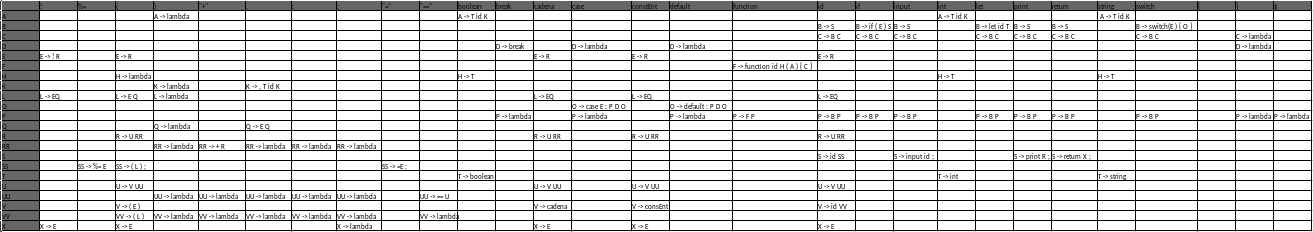
\includegraphics[width=1\textwidth]{tablaM.png}}
\caption{\label{figura:automata}Tabla de Análisis de LL1.}
\end{figure}

\newpage
\begin{appendices}

\section{Casos de Prueba}

\subsection{Prueba Funcional 1}
Código fuente:
\lstinputlisting[language=JavaScript]{p1.txt}
\hspace{\parindent} Fichero de Tokens:
\lstinputlisting[language=JavaScript]{p1T.txt}
\hspace{\parindent} Tabla de Símbolos:
\lstinputlisting[language=JavaScript]{p1TS.txt}

Como podemos ver en este caso el analizador léxico logra generar bien los tokens del fichero,
saltándose las líneas en blanco, y generando los id correspondientes a las variables que va
encontrando a lo largo del fichero: como ocurre con el entero ‘a’, la variable “cadena” y la
variable “SSSadena”. A su vez va generando los identificadores en la tabla de símbolos correctamente.

\subsection{Prueba Funcional 2}
Código fuente:
\lstinputlisting[language=JavaScript]{p2.txt}
\hspace{\parindent} Fichero de Tokens:
\lstinputlisting[language=JavaScript]{p2T.txt}
\hspace{\parindent} Tabla de Símbolos:
\lstinputlisting[language=JavaScript]{p2TS.txt}
\hspace{\parindent} En este otro ejemplo podemos ver que funciona perfectamente teniendo comentarios de bloque tanto al inicio, al final y entre medias del código, a su vez que comprobamos que se
generan bien los tokens del switch case. A su vez podemos comprobar que se generó bien la
tabla de símbolos.

\subsection{Prueba Funcional 3}
Código fuente:
\lstinputlisting[language=JavaScript]{p3.txt}
\hspace{\parindent} Fichero de Tokens:
\lstinputlisting[language=JavaScript]{p3T.txt}
\hspace{\parindent} Tabla de Símbolos:
\lstinputlisting[language=JavaScript]{p3TS.txt}
\hspace{\parindent} En este caso podemos observar el correcto funcionamiento de las palabras reservadas function, break y input. Además de poder ver el correcto guardado de los identificadores de la función en la tabla de símbolos, y la generación de tokens de negación.

\subsection{Prueba No Funcional 1}
Código fuente:
\lstinputlisting[language=JavaScript]{p4.txt}
\hspace{\parindent} Fichero de Tokens:
\lstinputlisting[language=JavaScript]{p4T.txt}
\hspace{\parindent} Tabla de Símbolos:
\lstinputlisting[language=JavaScript]{p4TS.txt}
\hspace{\parindent} En este ejemplo comprobamos si se detecta el error en la asignación con resto, ya que el \% debe llevar después un =, si no, el automata no lo reconoce.

\subsection{Prueba No Funcional 2}
Código fuente:
\lstinputlisting[language=JavaScript]{p5.txt}
\hspace{\parindent} Fichero de Tokens:
\lstinputlisting[language=JavaScript]{p5T.txt}
\hspace{\parindent} Tabla de Símbolos:
\lstinputlisting[language=JavaScript]{p5TS.txt}
\hspace{\parindent} Aquí comprobamos que la cadena numérica introducida no supere el valor máximo de 32767.

\subsection{Prueba No Funcional 3}
Código fuente:
\lstinputlisting[language=JavaScript]{p6.txt}
\hspace{\parindent} Fichero de Tokens:
\lstinputlisting[language=JavaScript]{p6T.txt}
\hspace{\parindent} Tabla de Símbolos:
\lstinputlisting[language=JavaScript]{p6TS.txt}
\hspace{\parindent} En este código vemos como trata el analizador léxico una cadena que sobrepasa el máximo permitido (64), se puede observar que no genera el token cadena.

\end{appendices}

\end{document}
